
 
  \chapter{Implementação \emph{web}} \label{CHP:RAILS}%%
	Conforme citado no capítulo \ref{CHP:FUND}, utilizaremos o \emph{framework} \emph{web} chamado Ruby on Rails, implementado sobre a linguagem Rails.
    \section{Ambientação}
     
    Para a configuração do ambiente Ruby on Rails, foram utilizadas as soluções de \cite{railsinstaller}, que implementou facilitadores para instalação em ambientes Windows e OS X. Porém, os aplicativos necessários podem ser instalados separadamente. Os necessários para a nossa aplicação foram:
\begin{itemize}
\item Ruby 1.9.3 -Interpretador da linguagem Ruby
\item Rails 3.2.11 - Pacote contendo todo o \emph{framework} Rails utilizado
\item Git 1.7.10 - Controlador de versão Git. Utilizamos para o controle da versão junto ao GitHub e para fazer o \emph{deploy}\footnote{\emph{Deploy} ou publicação é a instalação da aplicação em um servidor de aplicações.} no Heroku
\item RVM1.16.17 - Gerenciador de versões Ruby
\item Bundler 1.2.1 - Controle de dependências (Gems\footnote{Gems são pacotes que contém toda informação de arquivos a serem instalados.})
\end{itemize}     
    
	Uma das decisões mais importantes no processo de manufatura de uma aplicação é a escolha da ferramenta ideal de desenvolvimento, que forneça agilidade e os recursos necessários para o desenvolvedor.
	
    Por ser uma aplicação em Ruby, onde os arquivos de código e de configuração são baseados em texto puro, o \emph{Ruby on Rails} não exige nenhuma ferramenta avançada de criação. Em outras palavras, utilizar um editor de texto simples ou uma \ac{IDE} é uma decisão pessoal.
	
    As IDE's mais comuns para se trabalhar com \emph{Rails} são:
\begin{itemize}
\item RubyMine - Intellij IDEA
\item Aptana Studio 3 - antes conhecida como RadRails, \emph{plugin} para Eclipse
\item Ruby in Steel- Visual Studio
\item NetBeans - (até a versão 6.9)
\end{itemize}     
    De acordo com \cite{caelum}, a maioria dos desenvolvedores Ruby on Rails não utiliza nenhuma \ac{IDE}, apenas um bom editor de texto e um terminal (ou \emph{prompt}) de comando aberto.  Algumas ferramentas de texto boas para esse propósito, junto aos sistemas operacionais que suportam, são as seguintes:
\begin{itemize}
\item TextMate -  Mac OS X
\item Sublime Text - Mac OS X, Linux, Windows
\item Gedit - Mac OS X, Linux
\item Notepad++ - Windows
\item VI/Vim - Mac OS X, Linux, Windows
\end{itemize}
    Nesse projeto foi utilizado o TextMate, no ambiente Mac OS X.
    \section{Criação de aplicação}
            Uma vez que o \emph{Rails} tenha sido instalado corretamente e, automaticamente, definido como variável de ambiente no terminal, pode-se executar o comando ``rails'' para criação de aplicação e módulos.  Pode-se, também,  verificar a versão do rails através do comando:
			
\begin{lstlisting}
    $rails --version
\end{lstlisting}
           
    A versão utilizada nesse projeto foi a $3.2.11$, a última disponibilizada quando este texto foi escrito. A fim de criar a aplicação, utilizando o \ac{SGBD} PostgreSQL, foi executado o seguinte comando:
	\begin{lstlisting}
    $rails new iQuizzer -d postgresql
    \end{lstlisting}   
    Ao executar a última linha, o \emph{Rails} criou um diretório com alguns arquivos, que serão vistos na próxima seção.
     
    \section{Estrutura}
           
     
            Um projeto \emph{Rails} tem uma estrutura básica composta das seguintes pastas:
\begin{itemize}
\item App: contém os arquivos específicos da aplicação. Conforme citado no capítulo \ref{CHP:FUND}, o \emph{Rails} utiliza o padrão \ac{MVC}, e dentro desse diretório a divisão é feita através dos sub-diretórios \emph{model}, \emph{view} e \emph{controller};
\item Config: configurações diversas da aplicação;
\item db: contém as migrações (alterações no banco de dados durante o processo de desenvolvimento), além de alguns outros arquivos relacionados ao banco de dados;
\item doc: documentação do sistema;
\item lib: bibliotecas;
\item log: algumas informações de \emph{log};
\item public: nessa pasta estão contidos todos os arquivos públicos que serão servidos pela \emph{Web};
\item test: utilizado para testar a aplicação, normalmente quando se usa \ac{TDD}\footnote{Desenvolvimento orientado a testes é uma técnica de desenvolvimento de \emph{software} onde um caso de teste é escrito para cada funcionalidade a ser implementada.}. Neste projeto, não foi utilizado;
\item Tmp: arquivos temporários de sessão e \emph{cache};
\item Vendor: projetos dependentes (terceiros).
\end{itemize}     
     
    \section{Banco de dados}
    \subsection{PostgreSQL}
            Banco de dados são coleções de informações que se relacionam de forma que crie um sentido. Seu objetivo principal é representar abstratamente uma parte do mundo real, conhecida como ``Universo de Discurso'' \cite{ufmsbd}. 
			
    Na aplicação, foi utilizado um \ac{SGBD} relacional chamado PostgreSQL. Lançado em 1995, está atualmente na versão $9.1.4$, sobre a licença BSD\footnote{BSD foi criada pela Universidade de Berkeley e é conhecida por ser uma licença de pouca restrição quando comparada a GNU. Ela permite que o \emph{software} distribuído sobre a licença seja incorporado a produtos proprietários.}.
	
    A opção pela escolha do PostgreSQL deve-se ao bom suporte do Heroku a este \ac{SGBD}. Entretanto, outros motivos poderiam ser colocados em prol dessa decisão, a saber:
\begin{itemize}
\item Independência de plataforma - roda nos principais sistemas operacionais
\item Leve, podendo ser rodado em \emph{desktops} convencionais
\item Instalação simples
\item Gratuito
\end{itemize}
    \subsection{Modelos}
            Conforme o diagrama de classes citado na seção \ref{SEC:MER}, a aplicação possui algumas entidades, onde entidade é representada por uma tabela presente no banco de dados e um \emph{active record} contido na pasta app/models.
			
            O Rails possui uma forma bem simples de criar modelos, através de um comando de criação. Seja, por exemplo, a entidade ``Usuário'', tal que seus campos e tipos de campos sejam passados como parâmetros de um comando de criação de modelos:
			
\begin{lstlisting}
    $rails generate model Usuario nome:string sobrenome:string 
	apelido:string pontos_criador:float pontos_jogador:float 
	username:string senha:string
\end{lstlisting}
            A execução desse comando gera os seguintes arquivos:
\begin{itemize}
\item Um arquivo de migração de tabela, que cria a tabela usuário no banco de dados;
\item Uma classe chamada usuario.rb,  dentro de app/models,  e estende de ActiveRecord;
\item Arquivos de teste.

\end{itemize}     
    Após a criação do modelo, pode ser executado o seguinte comando:
	\begin{lstlisting}
    $rake db:migrate
     \end{lstlisting}
	 
    Esse comando tem a função de executar todas as migrações, ou seja, de alterar os dados no banco de dados. Caso seja necessária a modificação de um campo dessa tabela, como por exemplo, ao criar uma associação, pode ser criado um novo arquivo migration especificamente para isso.
	
    \subsection{Relacionamentos}
     
            Ao ser analisado o diagrama de classes da aplicação na seção \ref{SEC:MER}, pode-se verificar que existem relacionamentos entre as entidades apresentadas. Tais entidades representam relações entre tabelas do banco de dados, as quais devem ser implementadas na camada de modelo da aplicação.
			
            Para relacionar tais modelos, deve-se informar ao Rails o tipo de relacionamento existente. Isso é feito declarando o tipo de relacionamento entre modelos nos \emph{active records}. Os tipos de relacionamentos tratados são:
			
\begin{itemize}
\item $Belongs\_to$: é utilizado quando um modelo tem como atributo uma referência de outro modelo (em um relacionamento um para muitos ou um para um);
\item $has\_many$: associação contrária ao $belongs\_to$; indica que um determinado modelo tem muitas instancias de outro modelo;
\item $has\_one$: similar ao $has\_many$, porém com apenas uma instância (relacionamento um para um);
\item $has\_and\_belongs\_to\_many$: associação muitos para muitos.
\end{itemize}     

    As declarações de relacionamento criam alguns métodos de acesso automaticamente. Observe o código abaixo, do modelo de \emph{quiz} e do modelo de pergunta:
	
\begin{lstlisting}[language=Ruby]
    #-- classe Quiz
    class Quiz < ActiveRecord::Base
      	#modojogo: 1 - random, 2 - ordenate
    	attr_accessible :titulo, :perguntas_attributes, :modojogo,
		 :maxquestoes, :descricao, :usuario_id
     
    	 has_many :perguntas
    end
     
    #--classe Pergunta
    class Pergunta < ActiveRecord::Base
    	attr_accessible :conteudo, :respostas_attributes
     
    	belongs_to :quiz
    	has_many :respostas
    end
	
\end{lstlisting}

    Nesses modelos, foi definido que uma pergunta pertence a um \emph{quiz}, e que um \emph{quiz} possui várias perguntas. Tais definições criam métodos de acesso automaticamente, como:
	
\begin{lstlisting}   
	quiz.perguntas #retorna array de perguntas
	pergunta.quiz #retorna objeto Quiz
	
\end{lstlisting}     

    O \emph{Rails} não verifica automaticamente se a relação declarada funciona. Porém, de acordo com o princípio ``convenção sobre configuração'', definido no capítulo \ref{CHP:FUND}, é esperado que existam chaves estrangeiras do tipo \texttt{<modelo>\_id} nas tabelas que possuam relacionamentos do tipo $belongs\_to$. Para tanto, devemos criá-las nas tabelas do banco, utilizando um objeto \texttt{migration}\footnote{\emph{Migrations} são objetos em Ruby que realizam manipulações no banco, através de código SQL.}.
	
            Para criar um objeto \texttt{migration}, entre \emph{quiz} e perguntas, utilizou-se, por exemplo, o comando generate:
\begin{lstlisting}[language=Ruby]			
    Srails generate migration AddColumnQuizIdPergunta
 \end{lstlisting}   
       
    Isso gerou um arquivo \texttt{migration}  com o nome correspondente a $``<data\_hora> add\_column\_quiz\_id\_pergunta''$, no diretório /db/migrate. Implementou-se, então, o \texttt{migration} com o campo id:
	
\begin{lstlisting}[language=Ruby]
    classAddColumnQuizIdPergunta< ActiveRecord::Migration
    	def up
    	    add_column :Perguntas, :quiz_id, :integer
    	end
     
    	def down
    	end
    end
 \end{lstlisting}    
 
    Ao executar o \emph{script} de execução, $rake db:migrate$, será executado um SQL de criação da coluna no banco de dados. É recomendado que as alterações sofridas no banco de dados ao longo do projeto utilizem \texttt{migration}, uma vez que é possível registrar toda a seqüência de alterações no banco e reproduzi-las em outros ambientes.
     
     
    \section{Rotas e REST}
            As rotas no Rails servem para transformar determinadas requisições \ac{URL} em chamadas para controles particulares.  Algumas dessas rotas, para recursos, são utilizadas para o desenvolvimento da aplicação utilizando \ac{REST}, em conformidade ao definido no capítulo \ref{CHP:FUND}.
			
            Aplicações em \emph{Rails} são ditas \emph{RESTful}, associando o protocolo \ac{HTTP} às operações de \ac{CRUD}. Na aplicação, têm-se as seguintes operações disponíveis:
\begin{itemize}
\item \emph{Get}: retorna o valor ou representação do recurso - \emph{select};
\item \emph{Post}: criação de um novo recurso - \emph{insert};
\item \emph{Put}: altera o recurso - \emph{update};
\item \emph{Delete}: remove o recurso - \emph{delete}.
\end{itemize}     
    Para acessar o recurso, definimos uma rota de recurso no arquivo \texttt{routes.rb}. Seja o modelo de \emph{quiz}; define-se o seguinte recurso:
\begin{lstlisting}
    # routes.rb
    resources :quizzes
 \end{lstlisting}      
    Para esse recurso, o rails automaticamente cria sete rotas de acesso, a saber:
\begin{itemize}
\item GET /quizzes:controller => ' quizzes ', :action => 'index'
\item POST /quizzes:controller => ' quizzes ', :action => 'create'
\item GET /quizzes /new:controller => ' quizzes ', :action => 'new'
\item GET /quizzes /:id:controller => ' quizzes ', :action => 'show'
\item PUT /quizzes/:id:controller => 'quizzes ', :action => 'update'
\item DELETE /quizzes /:id:controller => ' quizzes ', :action => 'destroy'
\item GET /quizzes /:id/edit:controller => ' quizzes ', :action => 'edit'
\end{itemize}     

    Para todas as rotas criadas, o Rails também cria os \emph{helpers} (\emph{view} do \ac{MVC}):
	
\begin{itemize}
\item    $quizzes\_path         \# => "/quizzes "$
\item    $new\_quiz\_path      \# => "/quizzes /new"$
\item    $edit\_quiz\_path(3)  \# => "/quizzes /3/edit"$
\end{itemize}     
     
    Os resultados dos métodos invocados pelas rotas, por padrão, são em \ac{HTML}. Entretanto, existem facilitadores no \emph{Rails} para que esse retorno seja em \ac{XML} ou \ac{JSON}. Além disso, podemos passar no corpo de um \ac{HTTP} uma entrada em \ac{XML}/\ac{JSON}, de modo a ser interpretada pelo \emph{controller}.
	
            Na aplicação, toda a comunicação entre o \emph{Web Service} (aplicação \emph{Rails}) e o cliente (aplicação \emph{mobile}) é feita através de \ac{REST} utilizando \ac{JSON}. Isso é possível utilizando um \emph{format}\footnote{Os objetos \emph{respond\_to} são relativos ao tipo de requisição \ac{HTTP} que chega. Para cada tipo, uma variável \emph{format} é definida.}, como no exemplo abaixo:
\begin{lstlisting}[language=Ruby]
    # GET /quizzes
      # GET /quizzes.json
    def index
        @quizzes = Quiz.all
    	respond_to do |format|
          format.html # index.html.erb
          format.json { render :json => @quizzes }
   	   end
    end
     
 \end{lstlisting} 
 
            O método \texttt{index} é responsável por retornar um \emph{array} com todos os \emph{quizzes}. Se a requisição vier por \ac{HTML}, ou seja, do próprio \emph{site}, a resposta será em \ac{HTML}; caso contrario, a resposta será em \ac{JSON}. Dessa forma, percebemos que o modo como os dados são requisitados é que diferenciam a saída.
     
    \section{Autenticação}
            Conforme foi definido na seção \ref{SEC:RNF}, um dos requisitos não funcionais é a segurança, ou seja, o sistema deve ser capaz de garantir que os dados de cada usuário estejam protegidos.
			
            A autenticação de um usuário busca verificar a identidade digital do mesmo. A partir da autenticação, o sistema autoriza o acesso ou não a determinados recursos do sistema.
			
           Na aplicação, a autenticação é feita através de \emph{tokens}. \emph{Tokens} são chaves criptografadas que identificam uma sessão do usuário. Optou-se por disponibilizá-los no momento que o usuário realiza o \emph{login}. Uma vez que o navegador (ou o aplicativo móvel nativo) obtenha o \emph{token}, o acesso é garantido até que o mesmo expire.
			
            A fim de reduzir o tempo de desenvolvimento, utilizou-se uma \emph{gem}\footnote{As \emph{gems} são pacotes de arquivos Ruby com determinadas funcionalidades (\emph{plug-ins}.} chamada \emph{Devise}, para autenticação e gerência de contas. Essa \emph{gem} possui doze módulos para gerência de conta, dos quais foram utilizados os seguintes, com as funções de:
\begin{itemize}
\item \emph{Database authenticable}: encripta e armazena uma senha no banco de dados para validar a autenticidade de um usuário enquanto está logado;
\item \emph{Token Authenticable}: usuários permanecem logados enquanto um \emph{token} autenticado for válido;
\item \emph{Registerable}: permite ao usuário criar contas;
\item \emph{Recoverable}: gera uma nova senha para o usuário e o manda instruções para alterar sua senha;
\item \emph{Rememberable}: gerencia e limpa \emph{tokens} para lembrar o usuário de um \emph{cookie} já salvo;
\item \emph{Trackable}: guarda informações de acesso, como o número de vezes que o usuário realizou \emph{login}, o momento do último \emph{login} e o endereço IP;
\item \emph{Validatable}: Valida a conta através de email/senha.
\end{itemize}   
  
    O \emph{Devise} cria algumas telas (\emph{helpers}) por padrão. As telas de confirmação, envio de email, gerência de contas, senha e sessão são geradas de maneira básica. As imagens seguintes mostram algumas dessas telas, com o \emph{layout} modificado pelo \emph{Bootstrap}, que será abordado na próxima seção.
	 \begin{figure}[H]
	   % Requires \usepackage{graphicx}
	   \centering
	   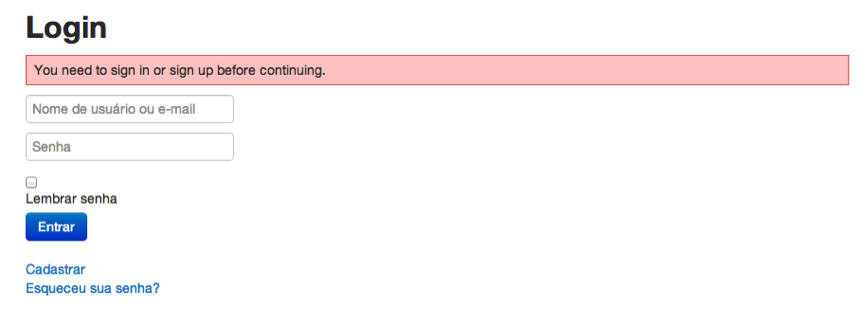
\includegraphics{figs/railslogin.png}\\
	   \caption{ Tela mostrada quando o usuario tenta acessar recurso e nao está logado }
	   \label{FIG:railslogin}
	 \end{figure}
	 
	 \begin{figure}[H]
	   % Requires \usepackage{graphicx}
	   \centering
	   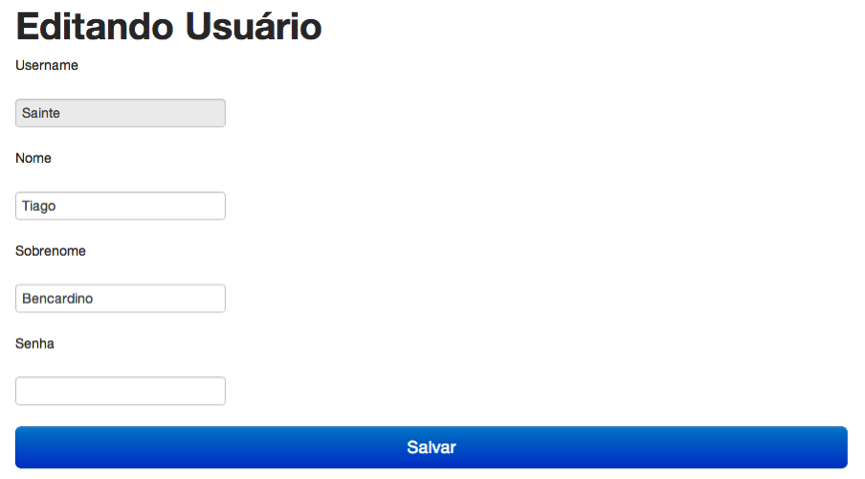
\includegraphics{figs/railsedituser.png}\\
	   \caption{ Edição de dados do usuário }
	   \label{FIG:railsuseredit}
	 \end{figure}
	 
	 \begin{figure}[H]
	   % Requires \usepackage{graphicx}
	   \centering
	   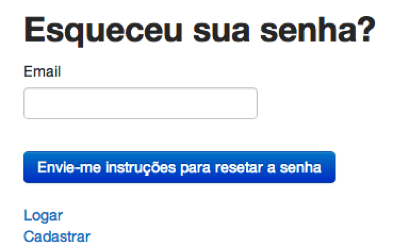
\includegraphics{figs/railsforgetpass.png}\\
	   \caption{ Lembrar senha do usuário }
	   \label{FIG:railsforgetpass}
	 \end{figure}

    Para a validação da sessão no \emph{mobile}, utilizamos essencialmente manipulação por \emph{tokens}. No momento que o usuário abre a aplicação, é verificado se o \emph{token} é válido: caso não seja, uma tela pedindo nome de usuário e senha é mostrada. Após o usuário fornecer os dados, é enviada uma requisição em \ac{JSON} para \url{/api/v1/token_controller}, que verifica se os dados estão corretos e se o usuário realmente existe. Se tudo ocorrer corretamente, um \emph{token} é retornado da requisição; caso contrário, uma mensagem contendo o erro é retornada.
	 \begin{figure}[H]
	   % Requires \usepackage{graphicx}
	   \centering
	   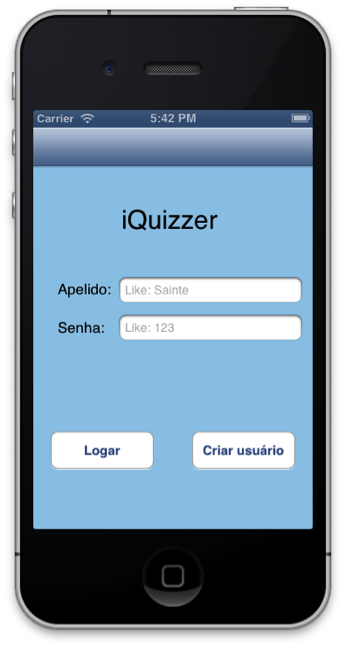
\includegraphics{figs/ioslogin.png}\\
	   \caption{ \emph{Login} no \emph{mobile} (iOS) }
	   \label{FIG:iOSlogin}
	 \end{figure}

    \section{\emph{Front-End}}
            No modelo \ac{MVC}, a parte de \emph{view} (visão) é responsável pelas interações com o usuário, recebendo as entradas e renderizando a saída. Os tipos de arquivos de fronteira mais comuns são o \ac{HTML}, ERB e o eRuby. Nessa aplicação, utilizou-se em quase todas as páginas a extensão ERB.
			
            Os \emph{controllers}, por sua vez, são responsáveis por receber a ação de uma \emph{view} e executar alguma lógica ligada a algum modelo. Basicamente, a função do \emph{controller} é de atender às requisições entre modelo e visão, fazendo toda a tradução necessária entre as camadas.
			
            Um \emph{controller} pode ser criado através de um comando \emph{generate}, como a seguir:
	\begin{lstlisting}
    $rails generate controller quizzes
    \end{lstlisting} 
            Esse comando irá criar uma classe chamada $quizzes\_controller.rb$ e uma pasta chamada \emph{quizzes}, dentro da pasta \emph{views}. A ligação entre as camadas é feita automaticamente, devido ao conceito de ``convenção sobre configuração''.
			
            Nesse \emph{controller} criado, foram colocados métodos de manipulação de dados (\emph{RESTful}). Na parte de visão, colocamos alguns arquivos para manipular \emph{quizzes}.  
			
            Veja, a seguir, o código da página \texttt{index.html.erb}. que tem como função listar \emph{quizzes} e navegar para tela de criação:
\begin{lstlisting}[language=HTML]
<h1>Quizzes</h1>
     
<table class="table table-hover">
    <thead>
        <tr>
            <th>#</th>
            <th> Titulo </th>
            <th> Descricao </th>
            <th> Criador </th>
            <th> #Perguntas </th>
        </tr>
    </thead>
    <tbody>
        <% @quizzes.each do |quiz| %>
            <tr>
                <td><%= quiz.id %></td>
                <td><%= link_to quiz.titulo, quiz %></td>
                <td><%= quiz.descricao %></td>
                <td><%= link_to quiz.user.username, quiz.user %></td>
                <td><%= quiz.perguntas.size %></td>
            </tr>
        <% end %>
    </tbody>
</table>
     
<%= link_to new_quiz_path do %>
    <button class="btn btn-large btn-block btn-primary" type="button">
        Criar quiz
    </button>
<% end %>
 \end{lstlisting} 
 
             Nesse código, é possível observar que existe código Ruby inserido entre os caracteres ``<\%'' e ``\%>''. Esses caracteres representam um escape do \ac{HTML} para  o Ruby. Quando colocado com um sinal de igual, ``<\%='', o resultado da linha executada é impressa na tela final \ac{HTML} apresentada ao usuário.
			 
            É importante observar que todos os atributos de classe do \emph{controller}, representados por um @, como em @quizzes, estão sobre o mesmo escopo.
			
    \subsection{\emph{Bootstrap}}
            ``Elegante, intuitivo e poderoso \emph{framework} de \emph{front-end} para desenvolvimento \emph{web} rápido e fácil'' - com essa descrição, o \emph{Bootstrap} é apresentado em seu \emph{site} oficial \cite{bootstrap}.  Lançado em Agosto de 2011 pelo Twitter, é atualmente o projeto mais popular do GitHub \cite{githubpop}.
			
            O \emph{Bootstrap} é uma coleção livre de ferramentas para desenvolver \emph{sites} e aplicações \emph{web}. Basicamente, contém \emph{templates} \ac{HTML}, JavaScript e \ac{CSS} para tipografia, formas, botões, gráficos, navegações e etc.
    Na aplicação, utilizamos o \emph{Bootstrap} para personalização de botões, tabelas, divisão da página em duas seções e menu.
	 \begin{figure}[H]
	   % Requires \usepackage{graphicx}
	   \centering
	   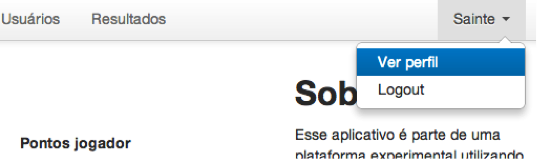
\includegraphics{figs/bootstrapcontrol.png}\\
	   \caption{ Exemplo de controle \emph{Bootstrap} }
	   \label{FIG:bootstrapcontrol}
	 \end{figure}
     
            Uma das funcionalidades mais aclamadas do \emph{Bootstrap} é a adequação da tela para resoluções menores: quando colocado em telas de pouca largura, tipicamente em \emph{smartphones}, a página se adéqua para ser apresentada em um \emph{layout} mais amigável para dispositivos móveis, como abaixo:
	 \begin{figure}[H]
	   % Requires \usepackage{graphicx}
	   \centering
	   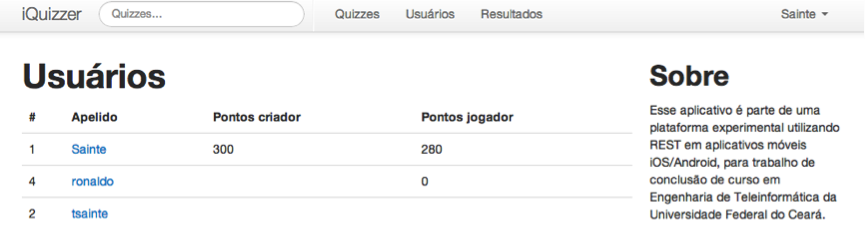
\includegraphics{figs/bootstraplayout1.png}\\
	   \caption{ Tela desktop extendida}
	   \label{FIG:bootstrapcontrol}
	 \end{figure}
	 
	 %%seria legal se ficassem lado a lado....
	 \begin{figure}[H]
	   % Requires \usepackage{graphicx}
	   \centering
	   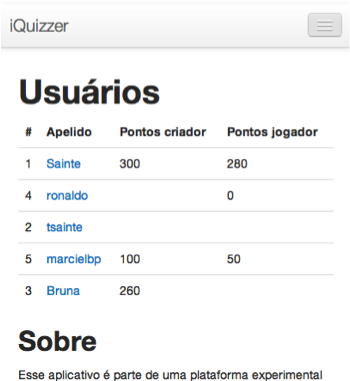
\includegraphics{figs/bootstraplayout2.png}\\
	   \caption{ Tela \emph{mobile} com menu suprimido }
	   \label{FIG:bootstrapcontrol}
	 \end{figure}
	 \begin{figure}[H]
	   % Requires \usepackage{graphicx}
	   \centering
	   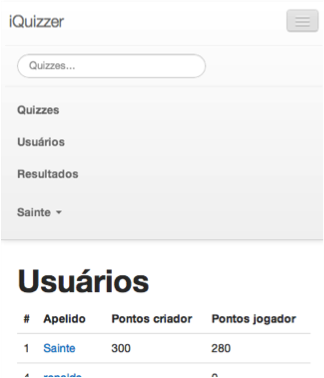
\includegraphics{figs/bootstraplayout3.png}\\
	   \caption{ Tela \emph{mobile} com menu extendido }
	   \label{FIG:bootstrapcontrol}
	 \end{figure}

     
     
    \section{\emph{Deploy}}
            Para que uma aplicação \emph{Rails} execute, é necessário um servidor de aplicação. Em ambiente de desenvolvimento, utilizou-se o Webrick, que é um servidor já embutido em todas as aplicações. Para executá-lo, basta abrir o terminal, navegar até o diretório raiz da aplicação e executar o seguinte comando:
			
	\begin{lstlisting}		
    rails server
     \end{lstlisting}
	 
            Caso uma porta diferente da porta padrão seja necessária (3000), pode ser passado o parâmetro -p xxxx, onde xxxx é a porta desejada.
			
            O ambiente de produção deste projeto está hospedado como serviço no Heroku, sobre a instância ``Celadon Cedar''. Para ativar, foi necessário fazer o cadastro, instalar o \emph{Heroku Toolbelt}, efetuar \emph{login} via terminal e fazer \emph{deploy}. Mais detalhes podem ser encontrados no QuickStart do Heroku \cite{quickheroku}.
			
            A submissão de arquivos para o servidor do Heroku é feita através do controlador de versão Git. Para submeter, deve-se realizar o \emph{commit}\footnote{O termo ``commit'' refere-se à ideia de fazer permanentes um conjunto de mudanças experimentais. Em um controlador de versão, é uma ação onde as alterações nos códigos são salvas, com uma descrição e colocadas em uma determinada versão.} do código e realizar um \texttt{git push}\footnote{O \texttt{git push} é um comando do Git para o envio de uma versão do projeto para um servidor git.} para o servidor. Caso seja necessário executar algum comando, como \emph{rake} de \emph{migrations}, usa-se o \texttt{run}, conforme a seguir:
			
\begin{lstlisting}	
    heroku run rake db:migrate 
\end{lstlisting}